
%(BEGIN_QUESTION)
% Copyright 2010, Tony R. Kuphaldt, released under the Creative Commons Attribution License (v 1.0)
% This means you may do almost anything with this work of mine, so long as you give me proper credit

Entreprenører installerer denne vortex-flowmåleren, utstyrt med pulsutgang (1 puls per 25 gallon), for å totalisere flow gjennom et rør:

$$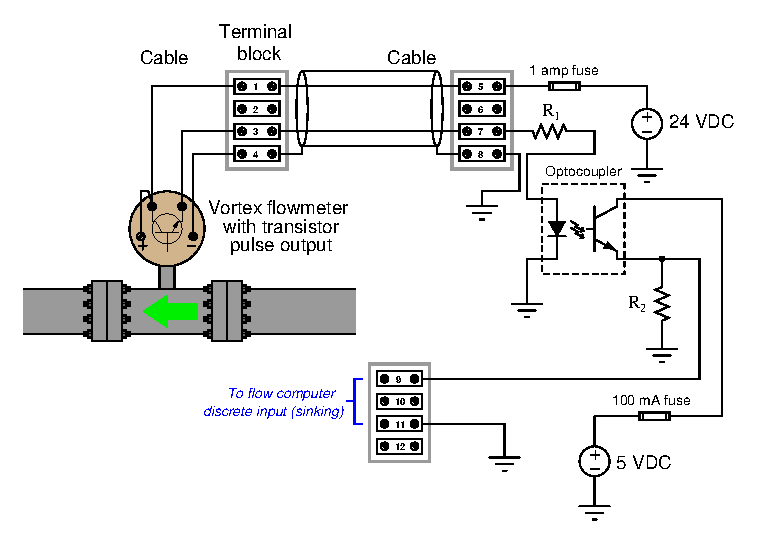
\includegraphics[width=15.5cm]{i00053x01.eps}$$

Dessverre registrerer ikke flow-computeren koblet til denne kretsen noen akkumulert mengde, selv om en operatør har verifisert flow i røret på omtrent 370 gallon per minutt.  Første steg er å koble fra flow-computerens inngang fra denne kretsen (slik at den er koblet nøyaktig som vist), og deretter måle DC-spenningen mellom terminal 1 og 4 med voltmeter: der viser måleren 23.1 volt DC.  Neste steg er å måle DC-spenningen mellom kollektor- og emitterterminalene på optokoblerens transistor: der viser måleren 0 volt.

Vurder sannsynligheten for hver spesifiserte feil i denne kretsen.  Vurder én feil om gangen (dvs. ingen samtidige feil), og avgjør om hver feil alene kan forklare {\it alle} målinger og symptomer i denne kretsen.

% No blank lines allowed between lines of an \halign structure!
% I use comments (%) instead, so that TeX doesn't choke.

$$\vbox{\offinterlineskip
\halign{\strut
\vrule \quad\hfil # \ \hfil & 
\vrule \quad\hfil # \ \hfil & 
\vrule \quad\hfil # \ \hfil \vrule \cr
\noalign{\hrule}
%
% First row
{\bf Feil} & {\bf Mulig} & {\bf Umulig} \cr
%
\noalign{\hrule}
%
% Another row
$R_1$ feilet åpen &  &  \cr
%
\noalign{\hrule}
%
% Another row
$R_2$ feilet åpen &  &  \cr
%
\noalign{\hrule}
%
% Another row
$R_1$ feilet kortsluttet &  &  \cr
%
\noalign{\hrule}
%
% Another row
$R_2$ feilet kortsluttet &  &  \cr
%
\noalign{\hrule}
%
% Another row
1 amp sikring sprengt &  &  \cr
%
\noalign{\hrule}
%
% Another row
100 milliamp sikring sprengt &  &  \cr
%
\noalign{\hrule}
%
% Another row
24 VDC kilde død &  &  \cr
%
\noalign{\hrule}
%
% Another row
5 VDC kilde død &  &  \cr
%
\noalign{\hrule}
} % End of \halign 
}$$ % End of \vbox

Til slutt, identifiser den {\it neste} diagnostiske testen eller målingen du ville gjort på dette systemet.  Forklar hvordan resultatet/resultatene av denne testen eller målingen hjelper deg å identifisere plasseringen og/eller naturen til feilen.

\vfil

\underbar{file i00053}
\eject
%(END_QUESTION)





%(BEGIN_ANSWER)


%(END_ANSWER)





%(BEGIN_NOTES)

% No blank lines allowed between lines of an \halign structure!
% I use comments (%) instead, so that TeX doesn't choke.

$$\vbox{\offinterlineskip
\halign{\strut
\vrule \quad\hfil # \ \hfil & 
\vrule \quad\hfil # \ \hfil & 
\vrule \quad\hfil # \ \hfil \vrule \cr
\noalign{\hrule}
%
% First row
{\bf Feil} & {\bf Mulig} & {\bf Umulig} \cr
%
\noalign{\hrule}
%
% Another row
$R_1$ feilet åpen &  & $\surd$ \cr
%
\noalign{\hrule}
%
% Another row
$R_2$ feilet åpen & $\surd$ &  \cr
%
\noalign{\hrule}
%
% Another row
$R_1$ feilet kortsluttet &  & $\surd$ \cr
%
\noalign{\hrule}
%
% Another row
$R_2$ feilet kortsluttet & $\surd$ &  \cr
%
\noalign{\hrule}
%
% Another row
1 amp sikring sprengt &  & $\surd$ \cr
%
\noalign{\hrule}
%
% Another row
100 milliamp sikring sprengt & $\surd$ &  \cr
%
\noalign{\hrule}
%
% Another row
24 VDC kilde død &  & $\surd$ \cr
%
\noalign{\hrule}
%
% Another row
5 VDC kilde død & $\surd$ &  \cr
%
\noalign{\hrule}
} % End of \halign 
}$$ % End of \vbox

Hvis $R_2$ var kortsluttet, ville det sprenge 100 mA-sikringen ved neste puls, og dermed skape 0 volt over optokoblerens C-E-terminaler.





\filbreak \vskip 20pt \vbox{\hrule \hbox{\strut \vrule{} {\bf Virtuell feilsøking} \vrule} \hrule}

\noindent
{\bf Predikere effekten av en gitt feil:} presenter hver av følgende feil til studentene, én om gangen, og la dem kommentere alle effekter hver feil vil gi.

\begin{itemize}
\item{} 
\item{} 
\item{} 
\end{itemize}


\vskip 10pt


\noindent
{\bf Identifisere mulige/umulige feil:} presenter symptomer til studentene og la dem deretter avgjøre om en serie foreslåtte feil kan forklare alle symptomene, og forklare {\it hvorfor} eller {\it hvorfor ikke} for hver foreslåtte feil:

\begin{itemize}
\item{} Symptom: {\it }
\item{}  -- {\bf Ja/Nei}
\item{}  -- {\bf Ja/Nei}
\item{}  -- {\bf Ja/Nei}
\end{itemize}


\vskip 10pt


\noindent
{\bf Vurdere nytte av gitte diagnostiske tester:} presenter symptomer til studentene og foreslå deretter følgende diagnostiske tester én etter én.  Studentene vurderer verdien av hver test og avgjør om den vil gi nyttig informasjon (dvs. fortelle oss noe vi ikke allerede vet).  Studentene avgjør hva ulike resultater for hver test eventuelt indikerer om feilen:

\begin{itemize}
\item{} Symptom: {\it Flow-computeren mottar et 5 volt DC-signal hele tiden, uavhengig av flow}
\item{} Mål spenning mellom terminal 1 og 3 -- {\bf Ja}
\item{} Mål spenning mellom terminal 5 og 8 -- {\bf Nei}
\item{} Sjekk 1 amp sikring -- {\bf Nei}
\item{} Mål spenning mellom terminal 7 og 8 -- {\bf Ja}
\item{} Mål resistans mellom terminal 9 og 11 -- {\bf Ja}
\item{} Sjekk 100 milliamp sikring -- {\bf Nei}
\item{} Mål 5 volt strømforsyningsutgang med voltmeter -- {\bf Nei}
\item{} Mål spenning mellom terminal 5 og 7 -- {\bf Ja}
\item{} Mål 24 volt strømforsyningsutgang med voltmeter -- {\bf Nei}
\end{itemize}


\vskip 10pt


\noindent
{\bf Diagnostisere en feil basert på gitte symptomer:} forestill deg at ??? feiler ??? i dette systemet (ikke avslør feilen til studentene!).  Presenter operatørens observasjon(er) til studentene, la dem vurdere mulige feil og diagnostiske strategier, og gi dem deretter resultatene av tester de foreslår basert på følgende symptomer, til de korrekt har identifisert feilens art og plassering:

\begin{itemize}
\item{} Operatørobservasjon: {\it }
\item{} 
\item{} 
\end{itemize}
%INDEX% Measurement, flow: vortex flow element
%INDEX% Troubleshooting review: electric circuits

%(END_NOTES)
